%%%%%%%%%%%%%%%%%%%%%%%%%%%%%%%%%%%%%%%%%%%%%%%%%%%%%%%%%%%%%%%
%                                                             %
%        DISTRIBUTED ANALYSIS NOTE                            %
%                                                             %
%       Author: Panos Christakoglou                           %
%               Markus Oldenburg                              %
%                                                             %
%       Last changes                                          %  
%  15.10.06: Summary and abstract by Markus                   %
%  22.12.06: Added the CAF reference                          %
%  22.12.06: Changes in Introduction.tex (Fed - Yves)         %
%  22.12.06: Changes in Flow.tex (Fed - Yves - Panos)         %
%  22.12.06: Changes in Local.tex (Fed - Yves - Panos)        %
%            Changing order (example comes first)             %    
%  23.12.06: Changes in Interactive.tex (Fed - Yves - Panos)  %
%            Changing order (example comes first)             %    
%  23.12.06: Changes in Batch.tex (Fed - Yves - Panos)        %
%                                                             %    
%%%%%%%%%%%%%%%%%%%%%%%%%%%%%%%%%%%%%%%%%%%%%%%%%%%%%%%%%%%%%%%
\documentclass[12pt,a4paper,twoside]{article}
\usepackage{indentfirst}
\usepackage{epsfig}
\usepackage[dvips]{color}
\usepackage{listings}
\lstset{                      % general command to set parameter(s)
  basicstyle=\ttfamily,       % print whole listing small
  keywordstyle=\bfseries,     % bold black keywords
  identifierstyle=,           % identifiers in italic
  commentstyle=\itshape,      % white comments in italic
  stringstyle=\ttfamily,      % typewriter type for strings
  showstringspaces=false,     % no special string spaces
  columns=fullflexible,       % Flexible columns
  xleftmargin=2em,            % Extra margin, left
  xrightmargin=2em,           % Extra margin, right
  numbers=left,               % Line numbers on the left
  numberfirstline=true,       % First line numbered
  firstnumber=1,              % Always start at 1 
  stepnumber=5,               % Every fifth line 
  numberstyle=\footnotesize\itshape, % Style of line numbers
  frame=lines}                % Lines above and below listings

\topmargin=1cm

\newcommand{\tag}{{\ttfamily Event Tag System }}

\begin{document}

\title{Distributed Analysis - Overview of the framework and practical examples}
\author{Editors: P.~Christakoglou\footnote{{\bf email : Panos.Christakoglou@cern.ch}}, M.~Oldenburg\footnote{{\bf email : Markus.Oldenburg@cern.ch}}}
\date{\today}

\maketitle

\begin{abstract}
In order to perform physics analysis in ALICE, a physicist has to use the GRID infrastructure since the data will be distributed in many sites. The machinery though complex due to the nature of the GRID, is totally transparent to the user who is shielded by a friendly user interface. In order to provide some guidelines to successfully utilize the provided functionalities, it was felt that an up-to-date manual was needed. With this document we try to explain the analysis framework as of today by covering all the recent developments.

After a short introduction, the general flow of a GRID based analysis will be outlined. The different steps of how to get your analysis ready and running on the GRID using the newly developed analysis framework will be covered in the subsequent chapters.


\end{abstract}

\newpage
\tableofcontents
%\lstlistoflistings


%________________________________________________________
\chapter{Introduction}
The intro to everything.
%________________________________________________________
%________________________________________________________
\section{Flow of the analysis procedure}
\label{Note:FLOW}

Fig.\,\ref{Note:FigAnalysisFlow} shows a schematic view of the flow of the analysis procedure. The first thing a typical user needs to do in order to analyze events stored on the GRID, is to interact with the file catalog in order to define the collection of files that he/she needs. This action implies the usage of the metadata fields assigned at the level of a run. Detailed description about the structure of the file catalog as well as the metadata fields on this level can be found in \cite{Note:RefFileCatalogMetadataNote,Note:RefFileCatalogMetadataWeb}. As an example, we have a user that wants to create a collection of tag files that fulfill the following criteria:

\begin{itemize}
\item The production year should be 2008.
\item The period of the LHC machine should be the first of 2008.
\item The data should come from the third reconstruction pass.
\item The collision system should be p+p.
\item The start and stop time of the run should be beyond the 19th of March 2008 and no later than 10:20 of the 20th of March 2008 respectively.
\end{itemize}

\noindent Then what needs to be written in the AliEn shell \cite{Note:RefFileCatalogMetadataWeb} (as a one line command) is:

\begin{lstlisting}[language=sh]
  find -x pp /alice/data/2008/LHC08a/*/reco/Pass3/* *tag.root 
  Run:collision_system=''pp'' and Run:stop<''2008-03-20 10:20:33'' 
  and Run:start>''2008-03-19'' > pp.xml
\end{lstlisting}

The previous lines imply the use of the {\ttfamily find} command of the alien shell \cite{Note:RefAlienTutorial}. The first argument of this command is the name of the collection which will be written inside the file. If the {\ttfamily -x pp} option is not used then we will not get back all the information about the file but instead we will just retrieve the list of logical file names (lfn). Then comes the path of the file catalog under which the files we want to analyze are stored followed by the name of the file. In this example, the path implies that the user requests a collection of real data ({\ttfamily /alice/data}) coming from the first period of the LHC machine in year 2008 ({\ttfamily /2008/LHC08a}), containing all the run numbers of the third pass of the reconstructed sample ({\ttfamily /*/reco/Pass3}). The last argument is the metadata fields: a variety of such fields can be combined using logical statements. The reader should notice that the output of this command is redirected to a xml file, which consists of all the necessary information (the file's unique identifier - guid, the logical file name etc) about the files that fulfill the imposed selection criteria. This xml collection, which is stored in the local and not the Grid working directory,  plays a very important role in the overall distributed analysis framework as we will see in the next sections. From the above example it is obvious that wild cards can be used.

Going back to the description of Fig.\,\ref{Note:FigAnalysisFlow} and following the flow of the arrows, we assume that the user creates a tag xml collection. Then in parallel inside a macro he/she imposes some selection criteria at the event level. Having those two components as an input, the \tag\ is queried and from this action, the system can either provide directly the input data collection, which is a chain of ESD files along with the associated event list (which describes the events that fulfill the imposed selection criteria), or a new ESD xml \footnote{This is different to the tag xml collection discussed earlier.} collection (mainly used for batch analysis --- see section \ref{Note:BATCH} for details). Even in the latter case, we end up having the chain along with the associated event list. This chain can then be processed by an analysis manager \cite{Note:RefAnalysisFramework} either locally, in AliEn \cite{Note:RefALIEN}, or using PROOF \cite{Note:RefPROOF}.

\begin{figure}[ht!]
\begin{center}
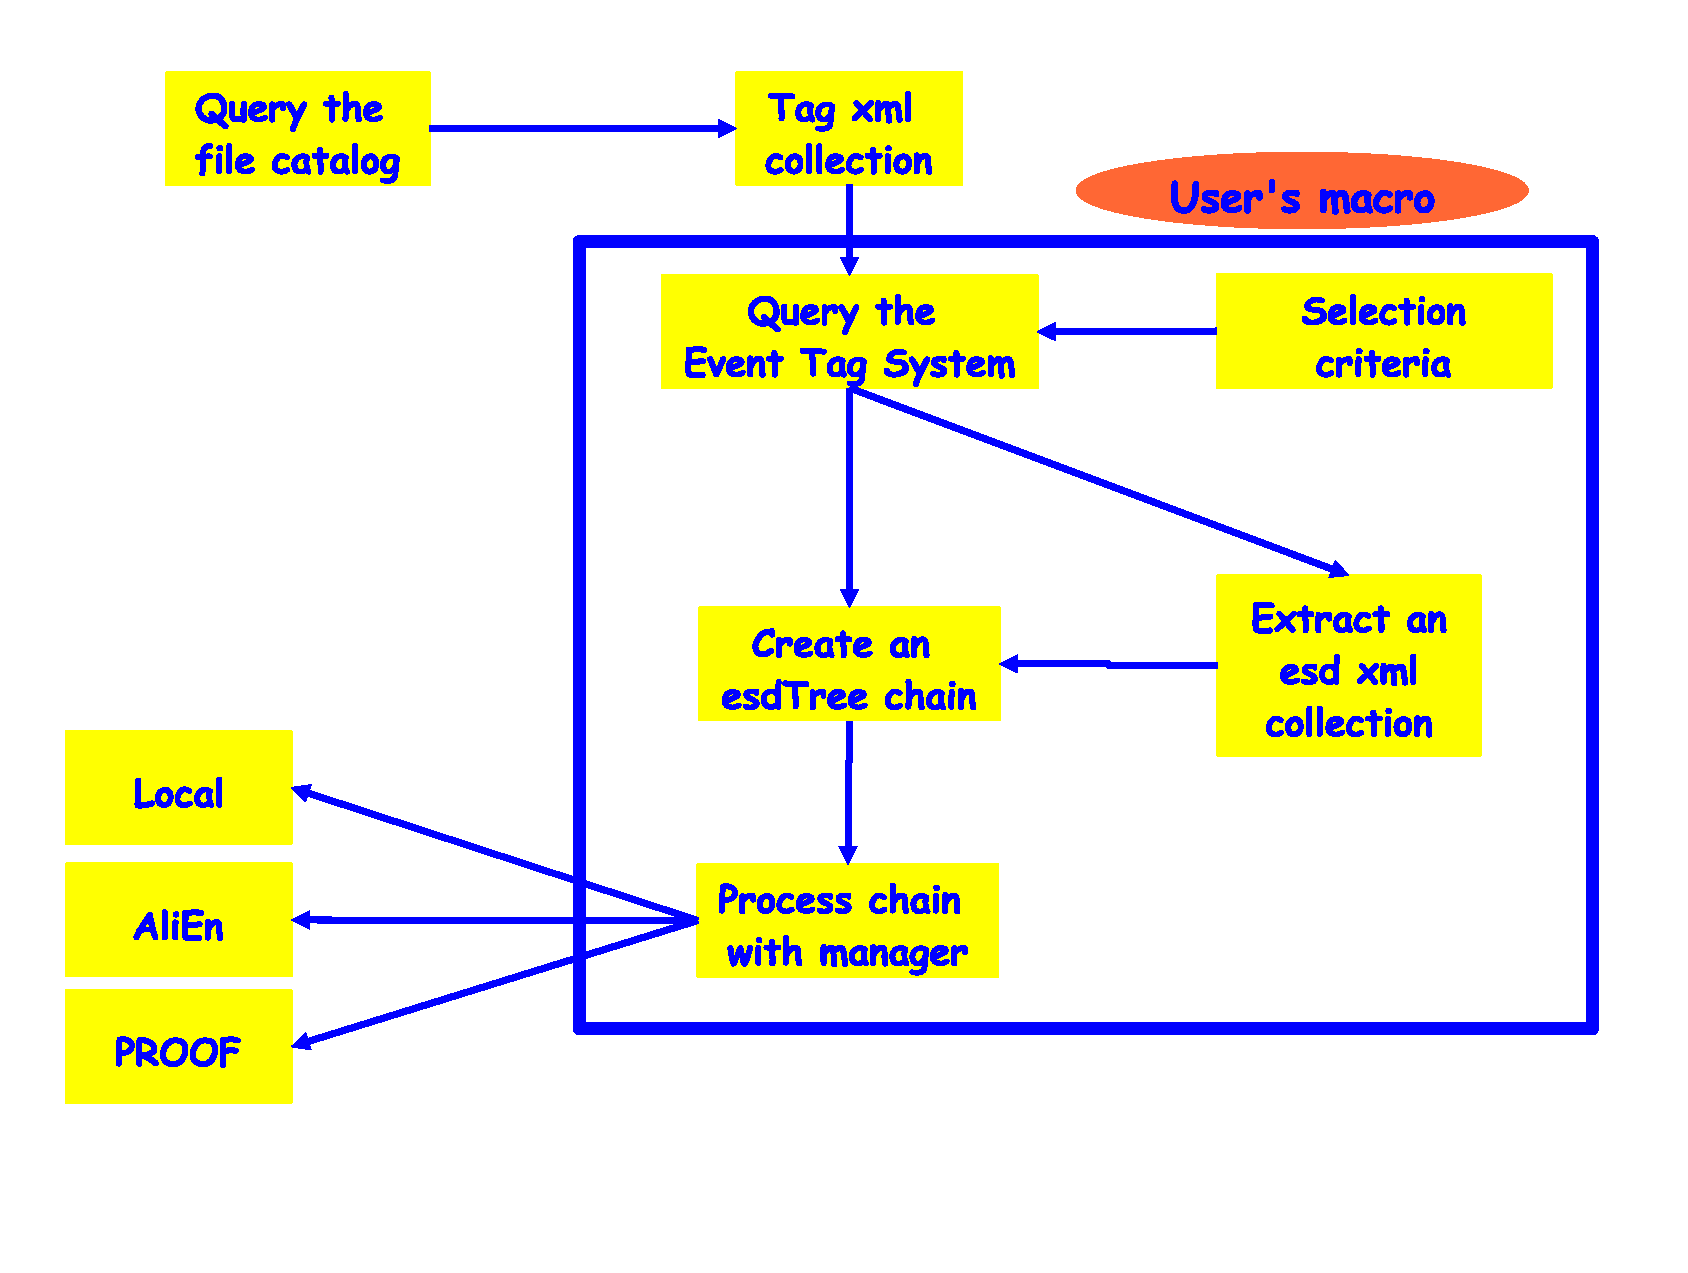
\includegraphics[width=0.7\textheight]{figures/Flow.eps}
\end{center}
\caption{The flow of the analysis procedure: Having as an input the tag xml collection that we create by querying the file catalog and the selection criteria, we interact with the \tag\ and we either get a chain along with the associated event list (events that fulfill the imposed selection criteria) or we create an ESD xml collection (for batch sessions) from which we create the ESD chain. This chain is processed with an analysis manager locally, in AliEn or even in PROOF.}
\label{Note:FigAnalysisFlow}
\end{figure}

We would also like to point out that we have two options on how to use the framework:

\begin{itemize}
\item We can work with aliroot and try all the examples that will be described in the next sections by loading all the corresponding libraries.
\item We can try to be as flexible as possible, by running ROOT along with the corresponding aliroot libraries (e.g. in the case of the analysis of AliESDs.root we need just the libESD.so along with the libANALYSIS\_NEW.so - the latter is needed for the new analysis framework which will be described in the next section). These libraries are created from the compilation of the relevant aliroot code which can be included in the so called {\ttfamily par file}. This par file is nothing more than a tarball containing the .h and .cxx aliroot code along with the Makefile and Makefile.arch (needed to compile the aliroot code in different platforms).
\end{itemize}

The user has these two possibilities although for some cases, like the analysis of generator information, the second option can't be used: we need to launch aliroot. In the following examples we will always concentrate in the case where we use the {\ttfamily par file}. The lines listed below show how we can setup, compile and load the libESD.so from the {\ttfamily ESD.par}.

\vspace{2 cm}

\begin{lstlisting}[language=C++]
  const char* pararchivename = "ESD";
  // Setup PAR File
  if (pararchivename) {
    char processline[1024];
    sprintf(processline,".! tar xvzf %s.par",pararchivename);
    gROOT->ProcessLine(processline);
    const char* ocwd = gSystem->WorkingDirectory();
    gSystem->ChangeDirectory(pararchivename);

    // check for BUILD.sh and execute
    if (!gSystem->AccessPathName("PROOF-INF/BUILD.sh")) {
      printf("*******************************\n");
      printf("*** Building PAR archive    ***\n");
      printf("*******************************\n");

      if (gSystem->Exec("PROOF-INF/BUILD.sh")) {
        Error("runProcess","Cannot Build the PAR Archive! - Abort!");
        return -1;
      }
    }
    // check for SETUP.C and execute
    if (!gSystem->AccessPathName("PROOF-INF/SETUP.C")) {
      printf("*******************************\n");
      printf("*** Setup PAR archive       ***\n");
      printf("*******************************\n");
      gROOT->Macro("PROOF-INF/SETUP.C");
    }
    
    gSystem->ChangeDirectory("../");
  }
  gSystem->Load("libVMC.so");
  gSystem->Load("libESD.so");
\end{lstlisting}


%________________________________________________________
%________________________________________________________
\section{Analysis framework}
\label{Note:ANALYSIS}

Recently, a new attempt has started that led to the development of a a new analysis framework \cite{Note:RefAnalysisFramework}. By the time this note was being written the framework has been validated in processes that concern this document (GRID analysis). We will review the basic classes and functionalities of this system in this paragraph (for further details the reader should look in \cite{Note:RefAnalysisFramework,Note:RefAlienTutorial}).

The basic classes that form this development are the following (we will give a full example of an overall implementation later):

\begin{itemize}
\item {\ttfamily AliAnalysisDataContainer:} The class that allows the user to define the basic input and output containers.
\item {\ttfamily AliAnalysisTask:} This is the class the lines of which should be implemented by the user. In the source file we can write the analysis code. 
\item {\ttfamily AliAnalysisManager:} Inside such a manager the user defines the analysis containers, the relevant tasks as well as the connection between them.
\end{itemize}

A practical example of a simple usage of this framework is given below where we extract a $P_{T}$ spectrum of all charged tracks (histogram) from an ESD chain (the examples can be found under the AnalysisMacros/Local/ directory of the PWG2 module of AliRoot).

\vspace{0.5 cm}
\textbf{AliAnalysisTaskPt.h}
\begin{lstlisting}[language=C++]
  #include "TH1.h"
  #include "AliESD.h"
  #include "AliAnalysisTask.h"

  class AliAnalysisTaskPt : public AliAnalysisTask {
    public:
    AliAnalysisTaskPt(const char *name);
    virtual ~AliAnalysisTaskPt() {}
    
    virtual void   Init(Option_t *);
    virtual void   Exec(Option_t *option);
    virtual void   Terminate(Option_t *);
    
    private:
    AliESD *fESD; //ESD object
    TH1F   *fHistPt; //Pt spectrum
    
    ClassDef(AliAnalysisTaskPt, 0); // example of analysis
  };
\end{lstlisting}

\vspace{0.5 cm}
\textbf{AliAnalysisTaskPt.cxx}
\begin{lstlisting}[language=C++]
  #define AliAnalysisTaskPt_cxx

  #include "TChain.h"
  #include "TH1.h"
  #include "TCanvas.h"
  #include "TSystem.h"
  #include "AliAnalysisTask.h"
  #include "AliESD.h"
  
  #include "AliAnalysisTaskPt.h"
  
  ClassImp(AliAnalysisTaskPt)
  
  //________________________________________________________________________
  AliAnalysisTaskPt::AliAnalysisTaskPt(const char *name) 
  :AliAnalysisTask(name,""), fESD(0), fHistPt(0) {
    // Constructor.
    // Input slot #0 works with a TChain
    DefineInput(0, TChain::Class());
    // Output slot #0 writes into a TH1 container
    DefineOutput(0, TH1F::Class());
  }
  
  //________________________________________________________________________
  void AliAnalysisTaskPt::Init(Option_t *) {
    printf("   Init %s\n", GetName());
    
    if (!fESD) {
      char ** address = (char **)GetBranchAddress(0, "ESD");
      if (address) fESD = (AliESD*)(*address);
      if (!fESD) {
	fESD = new AliESD();
	SetBranchAddress(0, "ESD", &fESD);
      }
      OpenFile(0,"Pt.ESD.1.root","RECREATE");
    }
    
    if (!fHistPt) {
      fHistPt = new TH1F("fHistPt","This is the Pt distribution",15,0.1,3.1);
      fHistPt->SetStats(kTRUE);
      fHistPt->GetXaxis()->SetTitle("P_{T} [GeV]");
      fHistPt->GetYaxis()->SetTitle("#frac{dN}{dP_{T}}");
      fHistPt->GetXaxis()->SetTitleColor(1);
      fHistPt->SetMarkerStyle(kFullCircle);
    }
  }
  
  //________________________________________________________________________
  void AliAnalysisTaskPt::Exec(Option_t *) {
    // Task making a pt distribution.
    // Get input data
    TChain *chain = (TChain*)GetInputData(0);
    Long64_t ientry = chain->GetReadEntry();
    if (!fESD) return;
    
    printf("Tracks: %d \n",fESD->GetNumberOfTracks());
    for(Int_t iTracks = 0; iTracks < fESD->GetNumberOfTracks(); iTracks++) {
      AliESDtrack * ESDTrack = fESD->GetTrack(iTracks);
      Double_t momentum[3];
      ESDTrack->GetPxPyPz(momentum);
      Double_t Pt = sqrt(pow(momentum[0],2) + pow(momentum[1],2));
      fHistPt->Fill(Pt);
    }//track loop 
    // Post final data. It will be written to a file with option "RECREATE"
    PostData(0, fHistPt);
  }      
  
  //________________________________________________________________________
  void AliAnalysisTaskPt::Terminate(Option_t *) {
    // Draw some histogram at the end.
    if (!gROOT->IsBatch()) {
      TCanvas *c1 = new TCanvas("c1","Pt",10,10,310,310);
      c1->SetFillColor(10);
      c1->SetHighLightColor(10);   
      c1->cd(1)->SetLeftMargin(0.15);
      c1->cd(1)->SetBottomMargin(0.15);  
      c1->cd(1)->SetLogy();
      fHistPt->DrawCopy("E");
    }
  }
\end{lstlisting}

The {\ttfamily AliAnalysisTaskPt} is a sample task that inherits from the {\ttfamily AliAnalysisTask} class. The main functions that need to be implemented are the following:

\begin{itemize}
\item Basic constructor: Inside the constructor we need to define the type of the input (if any input is to be used) as well as of the output of the task (in our example the input is of the form of a ROOT's {\ttfamily TChain} while the output is a histogram - {\ttfamily TH1F}).
\item {\ttfamily Init:} Inside this function we need to initialize the objects, assign the branch addresses to these objects, create the output file as well as the output histograms (as in our example) or objects.
\item {\ttfamily Exec:} The place where the analysis code should be implemented.
\item {\ttfamily Terminate:} The function inside of which we can draw histograms (as in our example) or perform any kind of actions (like merging of output).
\end{itemize}

\vspace{0.5 cm}
\textbf{Macro that creates an AliAnalysisManager}
\begin{lstlisting}[language=C++]
  //____________________________________________//
  // Make the analysis manager
  AliAnalysisManager *mgr = new AliAnalysisManager();
  //____________________________________________//
  // 1st Pt task
  AliAnalysisTask *task1 = new AliAnalysisTaskPt("TaskPt");
  mgr->AddTask(task1);
  // Create containers for input/output
  AliAnalysisDataContainer *cinput1 = mgr->CreateContainer("cchain1",
  TChain::Class(),AliAnalysisManager::kInputContainer);
  AliAnalysisDataContainer *coutput1 = mgr->CreateContainer("chist1", 
  TH1::Class(),AliAnalysisManager::kOutputContainer);
  
  //____________________________________________//
  mgr->ConnectInput(task1,0,cinput1);
  mgr->ConnectOutput(task1,0,coutput1);
  cinput1->SetData(chain1);
  
  if (mgr->InitAnalysis()) {
    mgr->PrintStatus();
    chain1->Process(mgr);
  }
\end{lstlisting}

\vspace{0.2 cm}
In the previous lines we firstly created a new analysis manager:\\
\\
{\ttfamily AliAnalysisManager *mgr = new AliAnalysisManager();}\\
\\
We then created a new {\ttfamily AliAnalysisTaskPt} object giving it a name and we assigned it to the manager:\\
\\
{\ttfamily AliAnalysisTask *task1 = new AliAnalysisTaskPt("TaskPt");}\\
{\ttfamily mgr->AddTask(task1);}\\
\\
Then the input and output containers were created while defining in parallel their types: \\
\\
{\ttfamily AliAnalysisDataContainer *cinput1 = mgr->CreateContainer("cchain1", TChain::Class(),AliAnalysisManager::kInputContainer);}\\
{\ttfamily AliAnalysisDataContainer *coutput1 = mgr->CreateContainer("chist1", TH1::Class(),AliAnalysisManager::kOutputContainer);}\\
\\
The next step was to link the task with the corresponding input and output container while setting the created chain of files (in the following section we will review how we can create this chain) to our input:\\
\\
{\ttfamily mgr->ConnectInput(task1,0,cinput1);}\\
{\ttfamily mgr->ConnectOutput(task1,0,coutput1);}\\
{\ttfamily cinput1->SetData(chain1);}\\
\\
Finally we process the chain with the manager:\\
\\
{\ttfamily   if (mgr->InitAnalysis()) chain1->Process(mgr);}\\

\vspace{0.5 cm}
In order for the user to have an idea of how the framework could look like in a complicated example, we provide figures \ref{Note:FigAnalysisFramework1} and \ref{Note:FigAnalysisFramework2}. In fig. \ref{Note:FigAnalysisFramework1} we show the flow of a typical analysis process:

A user interacts with the file catalog and creates a tag collection (the reader should check section \ref{Note:FLOW} for the instructions on how to perform this action). Then the \tag is queried (details on how we can do this will be provided in the next sections) and a chain of files is created. While looping the entries of this chain we split our analysis into two branches, on the first of which we analyze the (real or simulated) data and we provide as a last step an output ROOT file with histograms, while on the second we mix the events (event mixing method) in order to express our background. This second branch creates an output of the form of an Analysis Object Data (AOD) \cite{Note:RefComputingTDR}. A new chain is then created from this AOD and after analyzing the corresponding entries (analysis of mixed events) the output ROOT file with the relevant histograms is created. Finally, a last process is launched that compares the two output ROOT files and extracts the studied signal.


\begin{figure}[ht!]
\begin{center}
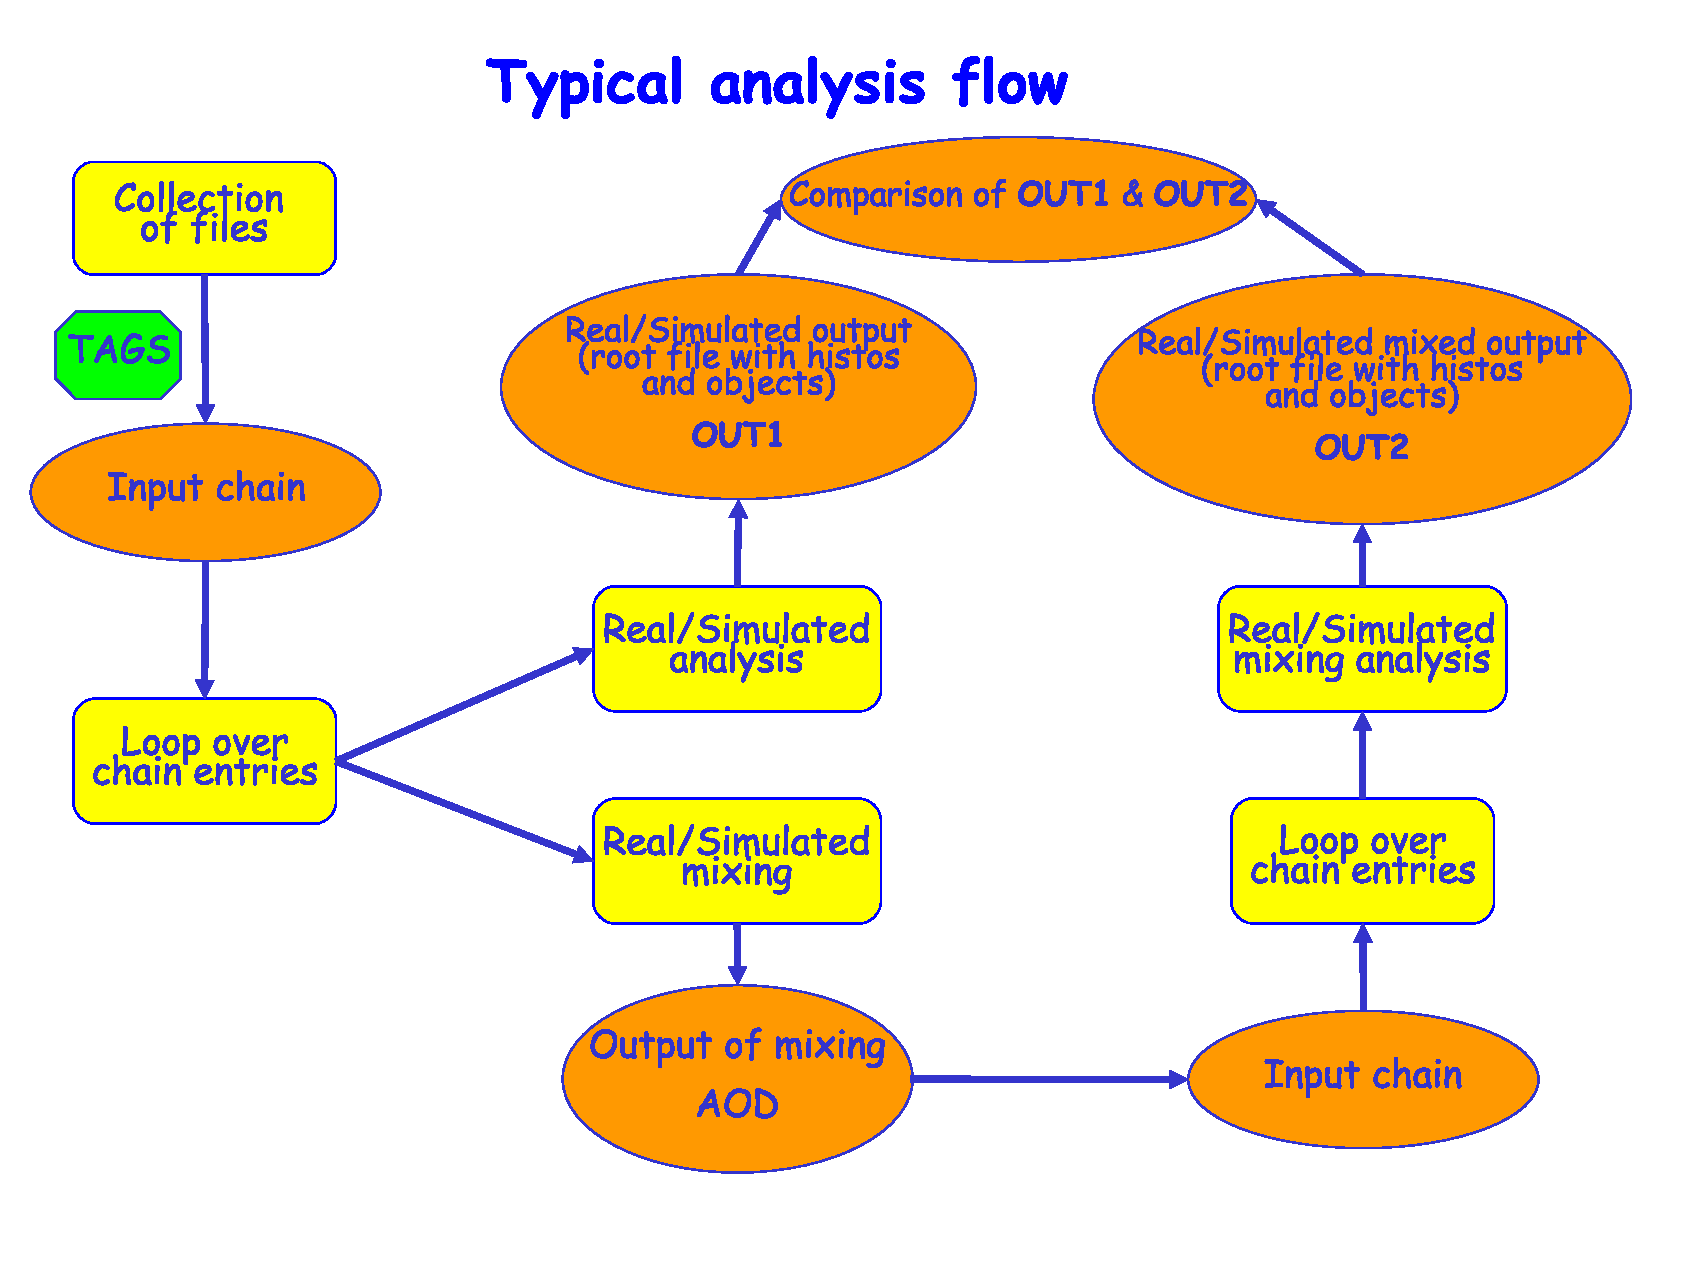
\includegraphics[width=15cm]{figures/AnalysisFramework-1.eps}
\end{center}
\caption{The flow of a typical physics analysis.}
\label{Note:FigAnalysisFramework1}
\end{figure}

\begin{figure}[ht!]
\begin{center}
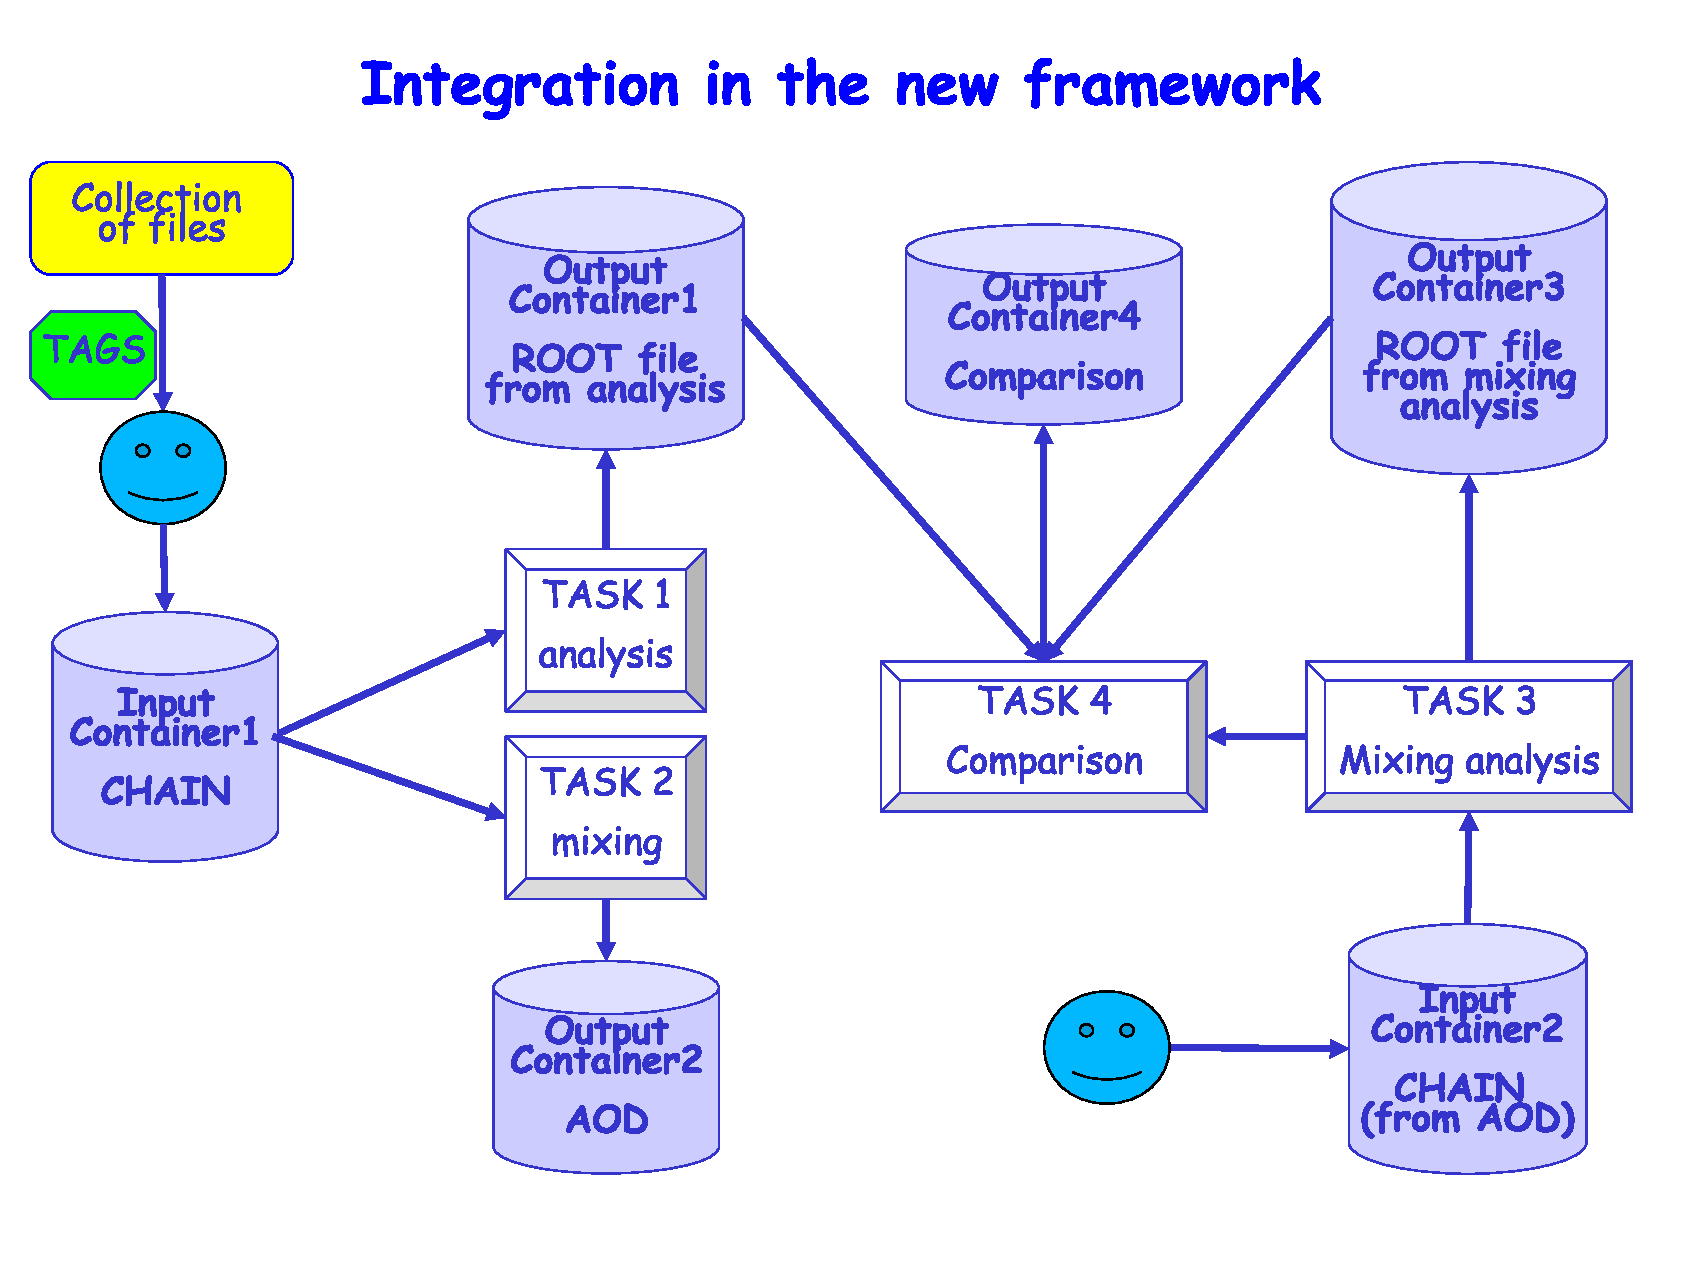
\includegraphics[width=15cm]{figures/AnalysisFramework-2.eps}
\end{center}
\caption{This figure shows how the physics analysis described in fig. \ref{Note:FigAnalysisFramework1} can be integrated in the new framework.}
\label{Note:FigAnalysisFramework2}
\end{figure}

Fig. \ref{Note:FigAnalysisFramework2} shows how we can integrate the previous use case to the new framework. The first steps are identical: A user interacts with the file catalog and creates a tag collection (as described in section \ref{Note:FLOW}) which is used as an input to query the \tag ~and create a chain of files. This chain is the first input container and is assigned to the {\ttfamily AliAnalysisManager}. In parallel we define two tasks which are also assigned to the manager and are both linked to the same input container (chain): the first analyzes the input data and creates an output container (ROOT file with histograms - signal + background plots), while the second is designed to mix the events and create a second output container (AOD). In order to analyze our mixed events, we initialize a second analysis manager which links the input container (AOD) with the new task (analysis of mixed events) and create a third output container (ROOT file with histogram - background plots). Finally the comparison task is added to the second manager. This task is triggered by the ending of the analysis of mixed events and takes two input containers (ROOT files having the signal + background plots and the pure background plots) while creating one output (extracted signal).

In the next paragraphs, we will be using the simplest possible case of manager and task which has been described in the beginning of this section.





%________________________________________________________
%________________________________________________________
\section{Interactive analysis with local ESDs}
\label{Note:LOCAL}

We assume that you have stored a few ESDs locally (the way to do this is described in detail in \cite{Note:RefAlienTutorial}) and that the first step regarding the creation of the tag files, which are also stored locally (under {\ttfamily path}), for these ESDs has been finished \cite{Note:RefEventTagNote}.

We setup the {\ttfamily par file} (see section \ref{Note:FLOW} for details) and then we invoke the following lines that summarize what we have to do  in order to analyze data stored locally using the \tag:\\

To specify cuts, we either do
\begin{lstlisting}[language=C++]
AliRunTagCuts *runCuts = new AliRunTagCuts();
runCuts->SetRunId(340);
// add more run cuts here...

AliEventTagCuts *evCuts = new AliEventTagCuts();
evCuts->SetMultiplicityRange(2, 100);
// add more event cuts here...
\end{lstlisting}
or we write
\begin{lstlisting}[language=C++]
const char *runCuts = "fAliceRunId == 340";
const char *evCuts = "fEventTag.fNumberOfTracks >= 2 &&
                      fEventTag.fNumberOfTracks <= 100";
// extend the strings to apply more cuts
\end{lstlisting}

Then we chain the tag files (keep in mind that the tag files in this example are stored locally under {\ttfamily path}), we query the \tag according to your cuts provided and we follow the example shown in section \ref{Note:ANALYSIS} to create a manager and a task:
\begin{lstlisting}[language=C++]
  AliTagAnalysis *tagAna = new AliTagAnalysis();
  tagAna->ChainLocalTags("path");
  TChain *analysisChain = tagAna->QueryTags(runCuts, evCuts);

  AliAnalysisManager *mgr = new AliAnalysisManager();
  AliAnalysisTask *task1 = new AliAnalysisTaskPt("TaskPt");
  mgr->AddTask(task1);

  AliAnalysisDataContainer *cinput1 = mgr->CreateContainer("cchain1",
  TChain::Class(),AliAnalysisManager::kInputContainer);
  AliAnalysisDataContainer *coutput1 = mgr->CreateContainer("chist1", 
  TH1::Class(),AliAnalysisManager::kOutputContainer);
  mgr->ConnectInput(task1,0,cinput1);
  mgr->ConnectOutput(task1,0,coutput1);
  cinput1->SetData(analysisChain);
  
  if (mgr->InitAnalysis()) {
    mgr->PrintStatus();
    analysisChain->Process(mgr);
  }

\end{lstlisting}

There are two possible ways to impose run and event cuts. The first is to create two objects, called {\ttfamily AliRunTagCuts} and {\ttfamily AliEventTagCuts}, whose member functions will take care of your cuts. The second is to provide two strings which describe the cuts you want to apply on the run and on the event level. In the following we will describe both methods.


\subsection{Object based cut strategy}
The first step in the object based cut strategy is to create an {\ttfamily AliRunTagCuts} and an {\ttfamily AliEventTagCuts} object:\\
\\
{\ttfamily AliRunTagCuts *runCuts = new AliRunTagCuts();}\\
{\ttfamily AliEventTagCuts *evCuts = new AliEventTagCuts();}\\
\\
These objects are used to describe the cuts imposed to your analysis, in order to reduce the number of runs and events to be analyzed to the ones effectively satisfying your criteria. There are many selections possible and they are provided as member functions of the two classes {\ttfamily AliRunTagCuts} and {\ttfamily AliEventTagCuts} class. In the case of the member functions describing a range of some entity, the run or event will pass the test if the described entity lies inclusively within the limits {\ttfamily low $\le$ value $\le$ high}. In case of only one argument, the run or event will pass the test if the entity is equal to the input flag or mask ({\ttfamily value == flag}, {\ttfamily value == mask}) or, in case of a 'Max' or 'Min' identifier, if the run or event quantity is lower or equal ({\ttfamily quantity $\le$ value}) or higher or equal ({\ttfamily quantity $\ge$ value}) than the provided value. A full list of available run and event cut functions can be found in Appendix\,\ref{App:ObjectCuts}.

Let's consider only a cut on the run number and one on the multiplicity: All events with run numbers others than 340 and all events with less than 2 and more than 100 particles will be discarded.\\
\\
{\ttfamily runCuts->SetRunId(340);}\\
{\ttfamily evCuts->SetMultiplicityRange(2, 100);}\\
\\
You can add as many other cuts as you like here.

\subsection{String based cut strategy}
Contrary to the object based cut strategy, you also have the possibility to provide your desired cut criteria as strings. You do that by creating two separate strings, one for the run cuts and one for the event cuts. The syntax is based on C and the string is later evaluated by the TTreeFormula mechanism of ROOT. Therefore a wide range of operators are supported (see the ROOT manual \cite{Note:ROOTManual} for details). The variables used to describe the run and event properties are the data members of the {\ttfamily AliRunTagCuts} and the {\ttfamily AliEventTagCuts} classes. Therefore they are same ones which are accessed by the object-based methods, but due to the enhanced number of available operators this system provides more flexibility.

In order to create the same cuts as in the object based example above, the two strings should look like this:\\
\\
{\ttfamily const char *runCuts = "fAliceRunId == 340";}\\
{\ttfamily const char *evCuts = "fEventTag.fNumberOfTracks >= 2 \&\&\\
fEventTag.fNumberOfTracks <= 100";}\\
\\
The full list of available data members to cut on can be found in Appendix\,\ref{App:StringCuts}. Within the quotes you can easily extend your cut statements in C style syntax.

\vspace{0.6cm}
Regardless of the way you choose to define your cuts, you create an {\ttfamily AliTagAnalysis} object, which is responsible to actually perform your desired analysis task.\\
\\
{\ttfamily AliTagAnalysis *TagAna = new AliTagAnalysis();}\\
\\
You have to provide this object with the locally stored tags since we assumed at the beginning of this section that these files were created and were stored locally (in the next section we will see how we can use the Grid stored tags). In order to do this you have to specify the correct path where the tag file(s) is/are located:\\ 
\\
{\ttfamily tagAna->ChainLocalTags("\emph{path}");}\\
\\
This function will pick up every file under the given path ending with {\ttfamily tag.root}. Now you ask your {\ttfamily AliTagAnalysis} object to return a {\ttfamily TChain}, imposing the event cuts as defined in the {\ttfamily AliRunTagCuts} and {\ttfamily AliEventTagCuts} objects or by the two strings representing the run and event tags:\\
\\
{\ttfamily TChain *analysisChain = tagAna->QueryTags(runCuts, evCuts);}\\
\\
The two arguments must be of the same type: two Ali*TagCuts objects or two strings! If you don't want to impose run or event cuts, simply provide a NULL pointer.

Finally you process the {\ttfamily TChain} by invoking your analysis manager with the following line of code:\\
\\
{\ttfamily  AliAnalysisManager *mgr = new AliAnalysisManager();}\\
{\ttfamily  AliAnalysisTask *task1 = new AliAnalysisTaskPt("TaskPt");}\\
{\ttfamily  mgr->AddTask(task1);}\\
{\ttfamily  AliAnalysisDataContainer *cinput1 = mgr->CreateContainer("cchain1", TChain::Class(),AliAnalysisManager::kInputContainer);}\\
{\ttfamily  AliAnalysisDataContainer *coutput1 = mgr->CreateContainer("chist1", TH1::Class(),AliAnalysisManager::kOutputContainer);}\\
{\ttfamily  mgr->ConnectInput(task1,0,cinput1);}\\
{\ttfamily  mgr->ConnectOutput(task1,0,coutput1);}\\
{\ttfamily  cinput1->SetData(analysisChain);}\\  
{\ttfamily  if (mgr->InitAnalysis()) analysisChain->Process(mgr);}\\

One thing to mention is that even in the case where you do not want to imply any run and event cuts, it is useful to use the chain of commands described above. You would then simply pass two {\ttfamily NULL} pointers to the {\ttfamily AliTagAnalysis} class. The advantage of this procedure is that this setup takes care of chaining all the necessary files for you.

All the needed files to run this example can be found inside the PWG2 module of AliRoot under the AnalysisMacros/Local directory.



%________________________________________________________
%________________________________________________________
\section{Interactive analysis with GRID ESDs}
\label{Note:INTERACTIVE}

Once the first step described in Section \ref{Note:LOCAL} was successful and we are satisfied from both the code and the results, we are ready to validate our code on a larger data sample. In this section we will describe how we can analyze interactively (that is sitting in from of a terminal and getting back the results in our screen) files that are stored in the Grid. We will once again concentrate in the case where we use the \tag\ \cite{Note:RefAlienTutorial,Note:RefEventTagWeb}.

The first thing that we need to create is a collection of tag files by querying the file catalog (for details on this process the reader should look either in the example of section \ref{Note:FLOW} or in \cite{Note:RefFileCatalogMetadataNote,Note:RefFileCatalogMetadataWeb}). These tag files, which are registered in the Grid, are the official ones created as a last step of the reconstruction code \cite{Note:RefEventTagNote}. Once we have a valid xml collection, we launch a ROOT session, we setup the {\ttfamily par file} (the way to do this has been described in detail in section \ref{Note:FLOW}), we apply some selection criteria and we query the \tag which returns the desired events in the proper format (TChain along with the associated list of events that satisfy our cuts). The following lines give a snapshot of how a typical code should look like:

\vspace{0.5 cm}
\textbf{Usage of AliRunTagCuts and AliEventTagCuts classes}
\begin{lstlisting}[language=C++]
  // Case where the tag files are stored in the file catalog
  // tag.xml is the xml collection of tag files that was produced 
  // by querying the file catalog.
  TGrid::Connect("alien://"); 
  TAlienCollection* coll = TAlienCollection::Open("tag.xml");
  TGridResult* tagResult = coll->GetGridResult("");

  // Create a RunTagCut object
  AliRunTagCuts *runCutsObj = new AliRunTagCuts();
  runCutsObj->SetRunId(340);

  // Create an EventTagCut object
  AliEventTagCuts *evCutsObj = new AliEventTagCuts();
  evCutsObj->SetMultiplicityRange(2, 100);

  // Create a new AliTagAnalysis object and chain the grid stored tags
  AliTagAnalysis *tagAna = new AliTagAnalysis(); 
  tagAna->ChainGridTags(tagResult);

  // Cast the output of the query to a TChain
  TChain *analysisChain = tagAna->QueryTags(runCutsObj, evCutsObj);

  // Process the chain with a manager
  AliAnalysisManager *mgr = new AliAnalysisManager();
  AliAnalysisTask *task1 = new AliAnalysisTaskPt("TaskPt");
  mgr->AddTask(task1);

  AliAnalysisDataContainer *cinput1 = mgr->CreateContainer("cchain1", 
  TChain::Class(),AliAnalysisManager::kInputContainer);
  AliAnalysisDataContainer *coutput1 = mgr->CreateContainer("chist1", 
  TH1::Class(),AliAnalysisManager::kOutputContainer);
  mgr->ConnectInput(task1,0,cinput1);
  mgr->ConnectOutput(task1,0,coutput1);
  cinput1->SetData(analysisChain);
  
  if (mgr->InitAnalysis()) {
    mgr->PrintStatus();
    analysisChain->Process(mgr);
  }
\end{lstlisting}

\vspace{0.5 cm}
\textbf{Usage of string statements}
\begin{lstlisting}[language=C++]
  // Case where the tag files are stored in the file catalog
  // tag.xml is the xml collection of tag files that was produced 
  // by querying the file catalog.
  TGrid::Connect("alien://"); 
  TAlienCollection* coll = TAlienCollection::Open("tag.xml");
  TGridResult* tagResult = coll->GetGridResult("");

  //Usage of string statements//
  const char* runCutsStr = "fAliceRunId == 340";
  const char* evCutsStr = "fEventTag.fNumberOfTracks >= 2 &&
  fEventTag.fNumberOfTracks <= 100";

  // Create a new AliTagAnalysis object and chain the grid stored tags
  AliTagAnalysis *tagAna = new AliTagAnalysis(); 
  tagAna->ChainGridTags(tagResult);

  // Cast the output of the query to a TChain
  TChain *analysisChain = tagAna->QueryTags(runCutsStr, evCutsStr);

  // Process the chain with a manager
  AliAnalysisManager *mgr = new AliAnalysisManager();
  AliAnalysisTask *task1 = new AliAnalysisTaskPt("TaskPt");
  mgr->AddTask(task1);

  AliAnalysisDataContainer *cinput1 = mgr->CreateContainer("cchain1",
  TChain::Class(),AliAnalysisManager::kInputContainer);
  AliAnalysisDataContainer *coutput1 = mgr->CreateContainer("chist1", 
  TH1::Class(),AliAnalysisManager::kOutputContainer);
  mgr->ConnectInput(task1,0,cinput1);
  mgr->ConnectOutput(task1,0,coutput1);
  cinput1->SetData(analysisChain);
  
  if (mgr->InitAnalysis()) {
    mgr->PrintStatus();
    analysisChain->Process(mgr);
  }
\end{lstlisting}


\noindent We will now review the previous lines. Since we would like to access Grid stored files we have to connect to the API server using the corresponding ROOT classes:\\
\\
{\ttfamily TGrid::Connect("alien://");}\\

Then we create a {\ttfamily TAlienCollection} object by opening the xml file (tag.xml) and we convert it to a {\ttfamily TGridResult}:\\
\\
{\ttfamily TAlienCollection* coll = TAlienCollection::Open("tag.xml");}\\
{\ttfamily TGridResult* tagResult = coll->GetGridResult("");}\\

\noindent where \textbf{tag.xml} is the name of the file (which is stored in the working directory) having the collection of tag files. 

The difference of the two cases is located in the way we apply the event tag cuts. In the first case, we create an {\ttfamily AliRunTagCuts} and an {\ttfamily AliEventTagCuts} object and impose our criteria at the run and event level of the \tag, while in the second we use the string statements to do so. The corresponding lines have already been descibe in the previous section. 


Regardless of the way we define our cuts, we need to initialize an {\ttfamily AliTagAnalysis} object and chain the GRID stored tags by providing as an argument to the {\ttfamily ChainGridTags} function the {\ttfamily TGridResult} we had created before:\\
\\
{\ttfamily AliTagAnalysis *tagAna = new AliTagAnalysis();}\\
{\ttfamily tagAna->ChainGridTags(tagResult);}\\

We then query the \tag, using the imposed selection criteria and we end up having the chain of ESD files along with the associated event list (list of the events that fulfill the criteria):\\
\\
{\ttfamily TChain *analysisChain = tagAna->QueryTags(runCutsObj, evCutsObj);}\\
\noindent, for the first case (usage of objects), or: \\
\\
{\ttfamily TChain *analysisChain = tagAna->QueryTags(runCutsStr, evCutsStr);}\\
\noindent, for the second case (usage of sting statements).

Finally we process this {\ttfamily TChain} by invoking our implemented task using a manager:\\
\\
{\ttfamily  AliAnalysisManager *mgr = new AliAnalysisManager();}\\
{\ttfamily  AliAnalysisTask *task1 = new AliAnalysisTaskPt("TaskPt");}\\
{\ttfamily  mgr->AddTask(task1);}\\
{\ttfamily  AliAnalysisDataContainer *cinput1 = mgr->CreateContainer("cchain1", TChain::Class(),AliAnalysisManager::kInputContainer);}\\
{\ttfamily  AliAnalysisDataContainer *coutput1 = mgr->CreateContainer("chist1", TH1::Class(),AliAnalysisManager::kOutputContainer);}\\
{\ttfamily  mgr->ConnectInput(task1,0,cinput1);}\\
{\ttfamily  mgr->ConnectOutput(task1,0,coutput1);}\\
{\ttfamily  cinput1->SetData(analysisChain);}\\  
{\ttfamily  if (mgr->InitAnalysis()) {mgr->PrintStatus();analysisChain->Process(mgr);}}\\

All the needed files to run this example can be found inside the PWG2 module of AliRoot under the AnalysisMacros/Interactive directory.


%________________________________________________________
%________________________________________________________
\section{Batch analysis}
\label{Note:BATCH}

In this section, we will describe the batch framework. We will first describe the flow of the procedure; we dedicate a sub-section to describe in detail the integration of the \tag in the batch sessions. We will then use the next paragraphs to describe in detail the files needed to submit a batch job as well as the jdl syntax. Finally we will provide a snapshot of a jdl and we will mention how we can submit a job on the grid and how we can see at any time its status.

%________________________________________________________
\subsection{Overview of the framework}

\begin{figure}[ht!]
\begin{center}
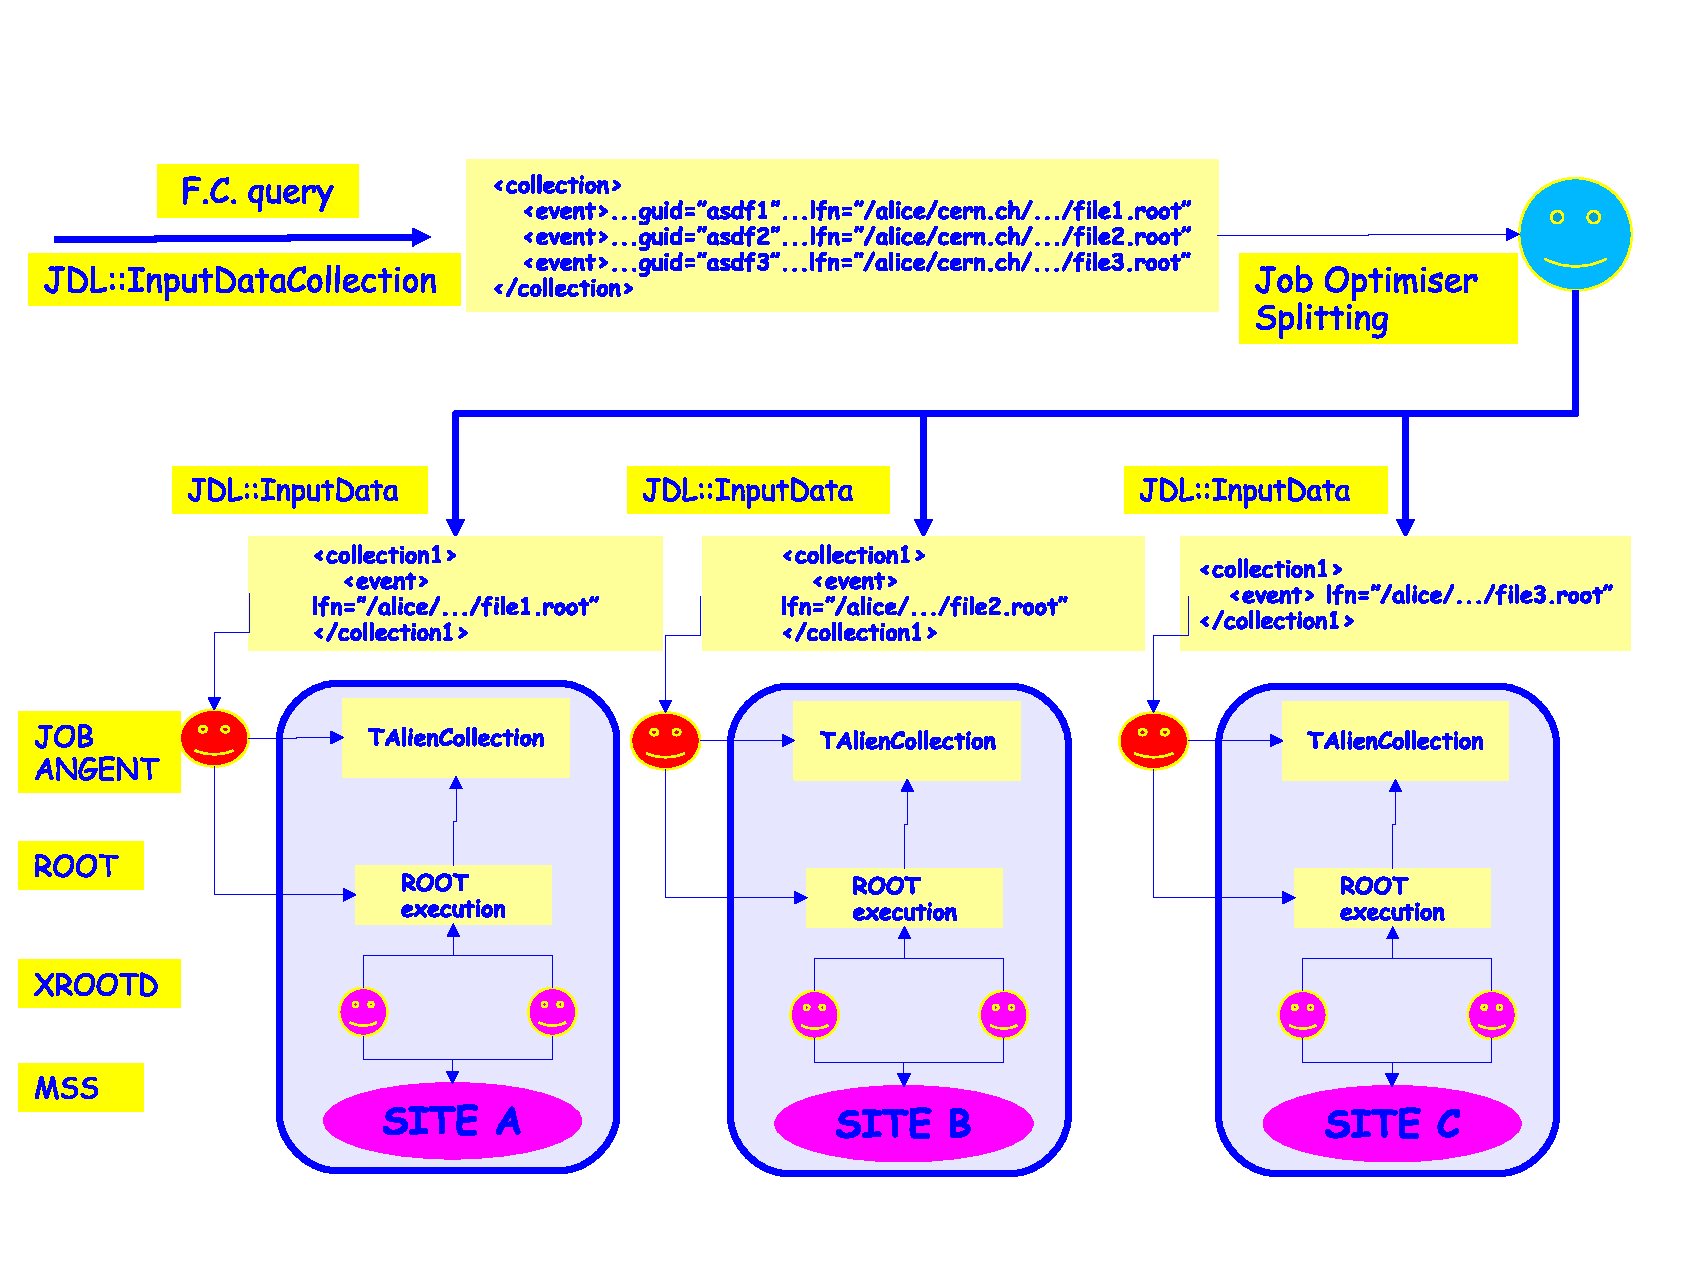
\includegraphics[height=0.5\textheight,width=0.7\textheight]{figures/Batch1.eps}
\end{center}
\caption{A schematic view of the flow of analysis in a batch session. Following the arrows, we have the initial xml collection which is listed in the jdl as an {\ttfamily InputDataCollection} field. The optimizer takes this xml and splits the master job into several sub-jobs while in parallel writing new xml collections on every worker node. Then the respective job agents on every site start a ROOT or AliRoot session, read these new xml collections and interact with the xroot servers in order to retrieve the needed files. Finally, after the analysis is completed, a single output file is created for every sub-job.}
\label{Note:FigAnalsysisFlowBatch}
\end{figure}

Fig.\,\ref{Note:FigAnalsysisFlowBatch} shows the flow of a batch session \cite{Note:RefAlienTutorial}. We start, as we have explained in section \ref{Note:FLOW}, by querying the file catalog and extracting a collection of files. This collection will be referenced by our jdl as an {\ttfamily InputDataCollection} field. Once we have created our jdl (a detailed description of the jdl syntax comes in the next sections) and all the files listed in it are in the proper place, we submit the job. The optimizer of the AliEn task queue parses the xml file and splits the master job into several smaller ones each one assigned to a different site. In parallel, a new xml collection is written on every site, containing the information about the files to be analyzed on every worker node.

The corresponding job agent of every site starts the execution of the ROOT (in case we use the combination ROOT + {\ttfamily par file}) or AliRoot session, parses this new xml collection and interacts with the xroot servers in order to retrieve from the storage system the files that are listed inside these collections. The analysis of these different sets of files results into the creation of several output files, each one containing the output of a sub-job. The user is responsible to launch a post process, that will loop over the different output files in order to merge them (an example on how to merge output histograms will be described in the next section).


%________________________________________________________
\subsection{Using the \tag}

To use the \tag, we have to use some {\ttfamily \textbf{AliRoot}} classes that are in the {\ttfamily \textbf{STEER}} module. The main classes, as described in a previous section (section \ref{Note:LOCAL}), are the {\ttfamily \textbf{AliTagAnalysis}}, {\ttfamily \textbf{AliRunTagCuts}} and {\ttfamily \textbf{AliEventTagCuts}}. In order to use the \tag in a batch session, we need to perform an initial step described in Fig.\,\ref{Note:FigAnalysisFlow}: starting from a tag xml collection obtained by querying the file catalog, we define our selection criteria according to our physics analysis and we create a new xml collection having this time the information about the AliESDs\footnote{The user should realize that the initial xml collection, named in the examples as {\ttfamily tag.xml}, held the information about the location of the tag files inside the file catalog. Instead what we create at this step is a new xml collection that will refer to the location of the ESD files.}. In this xml collection, we also list the events that satisfy the imposed selection criteria for every ESD file. The following lines show how we can generate a new xml collection (you can find these lines in the {\ttfamily \textbf{CreateXML.C}} macro inside the {\ttfamily \textbf{STEER}} module):

\vspace{0.5 cm}
\textbf{Usage of AliRunTagCuts and AliEventTagCuts classes}
\begin{lstlisting}[language=C++]
  // Case where the tag files are stored in the file catalog
  // tag.xml is the xml collection of tag files that was produced 
  // by querying the file catalog.
  TGrid::Connect("alien://"); 
  TAlienCollection* coll = TAlienCollection::Open("tag.xml");
  TGridResult* tagResult = coll->GetGridResult("");
  
  // Create a new AliTagAnalysis object
  AliTagAnalysis *tagAna = new AliTagAnalysis(); 

  // Create a tag chain by providing the TGridResult
  // from the previous step as an argument
  tagAna->ChainGridTags(tagResult);

  //Usage of AliRunTagCuts & AliEventTagCuts classes//
  // Create a RunTagCut object
  AliRunTagCuts *runCutsObj = new AliRunTagCuts();
  runCutsObj->SetRunId(340);

  // Create an EventTagCut object
  AliEventTagCuts *evCutsObj = new AliEventTagCuts();
  evCutsObj->SetMultiplicityRange(2, 100);

  // Create the esd xml collection:the first argument is the 
  // collection name while the other two are the imposed criteria
  tagAna->CreateXMLCollection("global", runCutsObj, evCutsObj);
\end{lstlisting}


\vspace{0.5 cm}
\textbf{Usage of string statements}
\begin{lstlisting}[language=C++]
  // Case where the tag files are stored in the file catalog
  // tag.xml is the xml collection of tag files that was produced 
  // by querying the file catalog.
  TGrid::Connect("alien://"); 
  TAlienCollection* coll = TAlienCollection::Open("tag.xml");
  TGridResult* tagResult = coll->GetGridResult("");
  
  // Create a new AliTagAnalysis object
  AliTagAnalysis *tagAna = new AliTagAnalysis(); 

  // Create a tag chain by providing the TGridResult
  // from the previous step as an argument
  tagAna->ChainGridTags(tagResult);

  //Usage of string statements//
  const char* runCutsStr = "fAliceRunId == 340";
  const char* evCutsStr = "fEventTag.fNumberOfTracks >= 2 &&
  fEventTag.fNumberOfTracks <= 100";

  // Create the esd xml collection:the first argument is the collection name 
  // while the other two are the imposed criteria 
  tagAna->CreateXMLCollection("global", runCutsStr, evCutsStr);
\end{lstlisting}

\noindent The reader should be familiar by now with the previous lines since they have already been described in detail in section \ref{Note:INTERACTIVE}. The new thing is the very last line of code where we call the {\ttfamily CreateXMLCollection} function of the {\ttfamily AliTagAnalysis} class which takes as arguments the name of the output xml collection (collection of ESDs) and the two run and event tag cuts (objects or strings). This output collection will be created in the working directory.

\begin{figure}[ht!]
\begin{center}
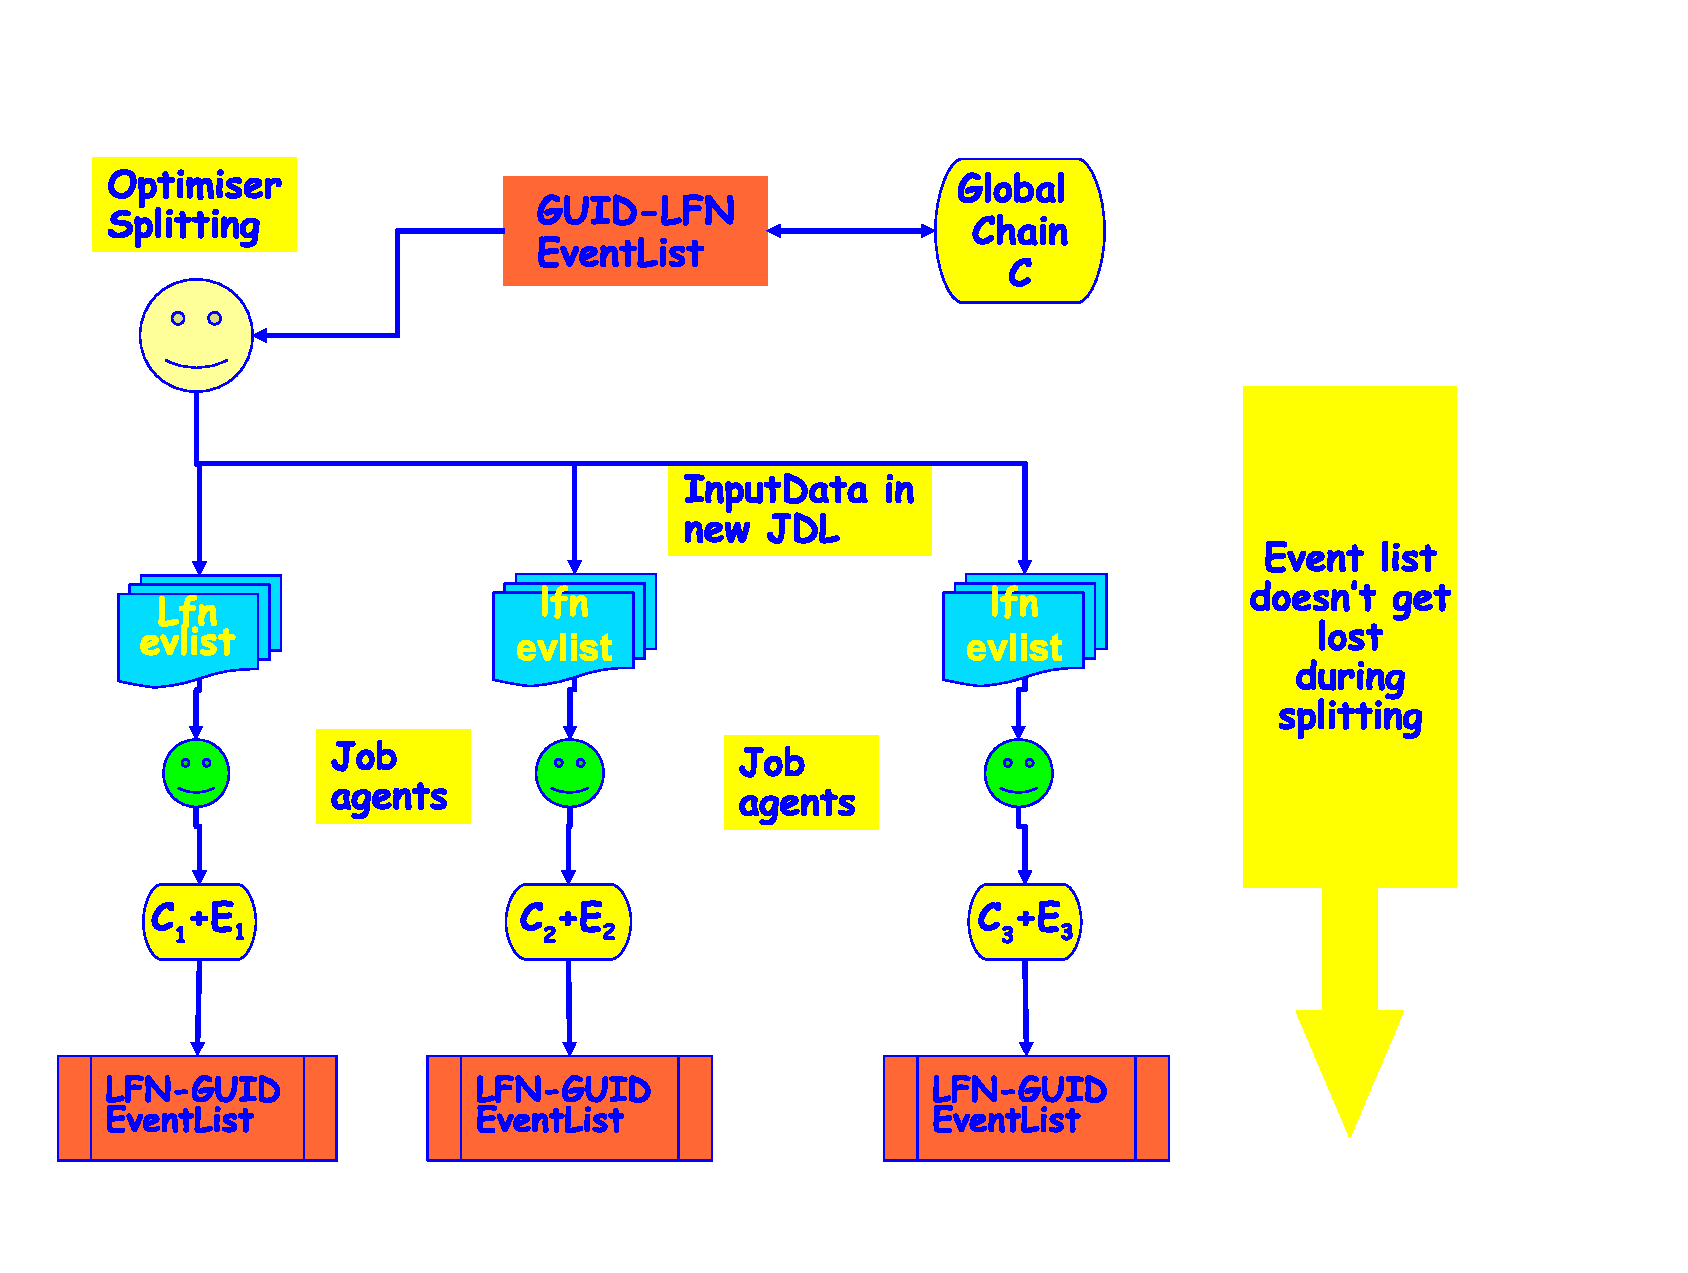
\includegraphics[width=0.7\textheight]{figures/Batch2.eps}
\end{center}
\caption{A schematic view of the flow of the analysis procedure in a batch session using the \tag. Following the arrows, we have the initial xml collection which is created by the {\ttfamily \textbf{AliTagAnalysis}} class listed in the jdl as an {\ttfamily \textbf{InputDataCollection}} field. The optimizer takes this xml once the master job is submitted and splits it into several sub-jobs while in parallel writing new xml collections on every worker node. These xml collections hold the information about the events that satisfy the imposed selection criteria, grouped by file: the analysis is performed only on these events on every worker node.}
\label{Note:FigAnalsysisFlowBatchTag}
\end{figure}

The next step will be, as in the previous section, to create a jdl file inside of which this newly created xml collection will be define as an {\ttfamily \textbf{InputDataCollection}} field. Then we once again submit the job and the optimizer parses the xml and splits the master job into several sub-jobs. In parallel, a new xml collection is written on every site, containing the information about the files that will be analyzed on every worker node as well as the corresponding list of events that satisfy the imposed selection criteria for every file. Thus, on every worker node we will analyze the created chain along with the associated event list as described in Fig.\,\ref{Note:FigAnalsysisFlowBatchTag}. Once finished, we will get several output files over which we will have to loop with a post process in order to merge them \cite{Note:RefAlienTutorial,Note:RefEventTagWeb}.

In the following paragraphs we will provide some practical information about the batch sessions, starting from the files needed to submit a job, what is the jdl syntax etc.

%________________________________________________________
\subsection{Files needed}

The files needed in order to submit a batch job are listed below \cite{Note:RefAlienTutorial}:

\begin{itemize}
\item \textbf{Executable}: This is a file that should be stored under the \$HOME/bin AliEn directory of each user. It is used to start the ROOT/AliRoot session on every worker node. Users can always use existing executables that can be found under /bin. An example is given below.
\item \textbf{Par file}: A {\ttfamily par file} is a tarball containing the header files and the source code of AliRoot, needed to build a certain library. It is used in the case where we do not want to launch aliroot but instead we want to be flexible by launching root along with the corresponding aliroot library (e.g root and the libESD.so). It is not compulsory although it is recommended to use a par file in an analysis.
\item \textbf{Macro}: It is the file that each user needs to implement. Inside the macro we setup the par file (in case we use it) and we load the needed libraries. Then we open the input xml collection and convert it into a chain of trees. Finally we process this chain with a selector. A snapshot of such a file has already been given in section \ref{Note:INTERACTIVE}.
\item \textbf{XML collection}: This is the collection created either by directly querying the file catalog (in the case where we don't use the \tag) or by querying the \tag (case described in the previous paragraph).
\item \textbf{JDL}: This is a compulsory file inside of which we should describe the input/output files as well as the packages that we are going to use. A detailed description about the JDL fields is provided in the next lines.
\end{itemize}

\textbf{Example of an ``executable''}
\begin{lstlisting}[language=bash]
  #!/bin/bash
  
  echo ===========================
  echo $PATH
  echo $LD_LIBRARY_PATH
  echo ==========================
  
  root -b -x runProcess.C;
\end{lstlisting}

%________________________________________________________
\subsection{JDL syntax}

In this section we will try to describe in detail the different jdl fields \cite{Note:RefGSHELL}.

\begin{itemize}
\item \textbf{Executable}: It is the only compulsory field of the JDL where we give the logical file name (lfn) of the executable that should be stored in /bin or \$VO/bin or \$HOME/bin. A typical syntax can be: \\{\ttfamily \textbf{Executable="balance.sh";}}.

\item \textbf{Packages}: The definition of the packages that will be used in the batch session. The different packages installed can be found by typing \textbf{packages} in the AliEn shell \cite{Note:RefGSHELL}. A typical syntax can be: \\{\ttfamily \textbf{Packages={"APISCONFIG::V2.2","ROOT::v5-13-04a"};}}.

\item \textbf{Jobtag}: A comment that describes the job. A typical syntax can be: \\{\ttfamily \textbf{Jobtag={"comment:Balance Function for pp@0.9TeV"};}}.

\item \textbf{InputFile}: In this field we define the files that will be transported to the node where the job will run and are needed for the analysis. A typical syntax can be: \\{\ttfamily \textbf{InputFile= {\\"LF:/alice/cern.ch/user/p/pchrist/Tutorial/BATCH/AliAnalysisTaskPt.cxx",\\"LF:/alice/cern.ch/user/p/pchrist/Tutorial/BATCH/AliAnalysisTaskPt.h",\\"LF:/alice/cern.ch/user/p/pchrist/Tutorial/BATCH/ESD.par", \\"LF:/alice/cern.ch/user/p/pchrist/Tutorial/BATCH/ANALYSIS\_NEW.par", \\"LF:/alice/cern.ch/user/p/pchrist/Tutorial/BATCH/demoBatch.C",\\"LF:/alice/cern.ch/user/p/pchrist/Tutorial/BATCH/runProcess.C"};}}.

\item \textbf{InputData}: This field, when defined, requires that the job will be executed in a site close to files specified here. This is supposed to be used in the case where you don't want to use a collection of files. It should be pointed out that it is not really practical because it implies that each user writes a large number of lines in the jdl, thus making it difficult to handle. It should be pointed out that this approach can be useful in the case where we use a few files. A typical syntax can be: \\{\ttfamily \textbf{InputFile= {\\"LF:/alice/cern.ch/user/p/pchrist/Tutorial/PDC06/001/AliESDs.root"}}}.

\item \textbf{InputDataList}: This is the name of the xml file created by the job agent after the job has been split, containing the lfn of the files of the closest storage element. A typical syntax can be: \\{\ttfamily \textbf{InputDataList="pp.xml";}}.

\item \textbf{InputDataListFormat}: The format of the previous field. It can be either ``xml-single'' where we imply that every xml entry corresponds to one file or ``xml-group'' where we imply that a new set of files starts every time the base filename appears (e.g. xml containing AliESDs.root, Kinematics.root, galice.root). In the context of this note, where we analyze only ESDs and not the generator information, we should use the first option. A typical syntax can be: \\{\ttfamily \textbf{InputDataListFormat="xml-single";}}. 

\item \textbf{OutputFile}: Here we define the files that will be registered in the file catalog once the job finishes. If we don't define the storage element, then the files will be registered in the default one which at the moment is Castor2 at CERN. A typical syntax can be: \\{\ttfamily \textbf{OutputFile={"stdout@ALICE::CERN::Castor2",\\"stderr@ALICE::CERN::Castor2","*.root@ALICE::CERN::Castor2"};}}. 

\item \textbf{OutputDir}: Here we define the directory in the file catalog under which the output files and archives will be stored. A typical syntax can be: \\{\ttfamily \textbf{OutputDir="/alice/cern.ch/user/p/pchrist/Balance/output";}}.

\item \textbf{OutputArchive}: Here we define the files that we want to be put inside an archive. It is recommended that the users use this field in order to place all their output files in such an archive which will be the only registered file after a job finishes. This is essential in the case of storage systems such as Castor which are not effective in handling small files. A typical syntax can be: \\{\ttfamily \textbf{OutputArchive={"logarchive:stdout,stderr,*.log@Alice::CERN::scratch",\\"rootarchive.zip:galice.root,geometry.root,Kinematics.root,\\TrackRefs.root,AliESDs.root,AliESDfriends.root,check.root,Run*.root\\@Alice::CERN::castor2"};}}.

\item \textbf{Validationcommand}: Specifies the script to be used as a validation script (used for production). A typical syntax can be: \\{\ttfamily \textbf{Validationcommand =\\"/alice/cern.ch/user/a/aliprod/prod2006/configspp/validation.sh";}}.

\item \textbf{Email}: If this field is defined, then you'll be informed that your job has finished from an e-mail. A typical syntax can be: \\{\ttfamily \textbf{Email="Panos.Christakoglou@cern.ch";}}.

\item \textbf{TTL}: One of the important fields of the JDL. It allows the user to define the maximum time in seconds the job will run. This field is used by the optimizer for the ordering and the assignment of the priority for each job. Lower value of TTL provides higher probability for the job to run quickly after submission. If the running time exceeds the one defined in this field, then the job is killed automatically. The value of this field should not exceed 100000 sec. A typical syntax can be: \\{\ttfamily \textbf{TTL = "21000";}}. 

\item \textbf{Split}: Used in the case we want to split our master job into several sub-jobs. Usually the job is split per storage element (se). A typical syntax can be: \\{\ttfamily \textbf{Split="se";}}.

\item \textbf{SplitMaxInputFileNumber}: Used to define the maximum number of files that will be analyzed on every worker node. A typical syntax can be: \\{\ttfamily \textbf{SplitMaxInputFileNumber="100";}}.

\end{itemize}

In summary, the following lines give a snapshot of a typical jdl:

\vspace{0.5 cm}
\textbf{Example of a JDL file}
\begin{lstlisting}[language=bash]
  # this is the startup process for root
  Executable="balance.sh";
  Jobtag={"comment:Balance Function for pp@0.9TeV"};
  
  # we split per storage element
  Split="se";
  
  # we want each job to read 100 input files
  SplitMaxInputFileNumber="100";
  
  # this job has to run in the ANALYSIS partition
  Requirements=( member(other.GridPartitions,"Analysis") );
  
  # we need ROOT and the API service configuration package
  Packages={"APISCONFIG::V2.2","ROOT::v5-13-04a"};

  # Estimation of the running time of the job
  TTL = "21000";
  
  # The xml file written by the job agent
  InputDataList="pp.xml";
  
  # ROOT requires the collection file in the xml-single format
  InputDataListFormat="xml-single";
  
  # This is our collection file containing the files to be analyzed
  InputDataCollection=
  "LF:/alice/cern.ch/user/p/pchrist/Balance/xml/pp900.xml,nodownload";
  
  # These are the input files that will be registered in the job's sandbox
  InputFile={
  "LF:/alice/cern.ch/user/p/pchrist/Tutorial/BATCH/AliAnalysisTaskPt.cxx",
  "LF:/alice/cern.ch/user/p/pchrist/Tutorial/BATCH/AliAnalysisTaskPt.h",
  "LF:/alice/cern.ch/user/p/pchrist/Tutorial/BATCH/ESD.par", 
  "LF:/alice/cern.ch/user/p/pchrist/Tutorial/BATCH/ANALYSIS_NEW.par", 
  "LF:/alice/cern.ch/user/p/pchrist/Tutorial/BATCH/demoBatch.C",
  "LF:/alice/cern.ch/user/p/pchrist/Tutorial/BATCH/runProcess.C"};
  
  # These are the files inside the output archive
  OutputArchive={"log_archive:stdout,stderr@Alice::CERN::se01",
    "root_archive.zip:*.root@Alice::CERN::castor2"};
  
  # Output directory
  OutputDir="/alice/cern.ch/user/p/pchrist/Balance/output";
  
  # email
  Email="Panos.Christakoglou@cern.ch";
  
\end{lstlisting}


%________________________________________________________
\subsection{Job submission - Job status}

After creating the jdl and registering all the files needed, we are ready to submit our batch job \cite{Note:RefGSHELL}. This can be done by typing: {\ttfamily \textbf{submit $<filename>$.jdl}} at the AliEn shell prompt. If there is no mistake in our JDL, the job will be assigned a JOBID. We can always see what are the jobs submitted by a certain user by typing {\ttfamily top -user $<username>$}. Later on, we can check its status by typing: {\ttfamily \textbf{ps -trace $<JOBID>$}}. The different states are:

\begin{itemize}

\item \textbf{INSERTING}: The job is waiting to be processed by the optimizer.
\item \textbf{SPLITTING}: The optimizer starts splitting the job if this is requested in the JDL.
\item \textbf{SPLIT}: Several sub-jobs were created from the master job.
\item \textbf{WAITING}: The job is waiting to be assigned to a job agent that fulfills its requirements.
\item \textbf{ASSIGNED}: A job agent is about to pick up this job.
\item \textbf{STARTED}: The job agent is preparing the input sandbox and transferring the files listed in the {\ttfamily \textbf{InputFile}} field.
\item \textbf{RUNNING}: The executable has started running.
\item \textbf{SAVING}: The executable has finished running and the job agent saves the output to the specified storage elements.
\item \textbf{SAVED}: The agent has successfully stored all the output files which are not available yet in the file catalog.
\item \textbf{DONE}: The central optimizer has registered the output in the catalog.

\end{itemize}

Finally, as long as a job status has turned into \textbf{RUNNING}, a user can check its stdout and stderr by typing: {\ttfamily \textbf{spy $<JOBID>$ stdout}} and {\ttfamily \textbf{spy $<JOBID>$ stderr}} at the AliEn prompt.


%________________________________________________________
\subsection{Merging the output}

Assuming that everything worked out and that the status of the job we had submitted has turned to {\ttfamily DONE}, we are ready to launch the post process that will access the different output files from every sub-job and merge them. We will concentrate in the case where the output files contain simple histograms (case which may represent the majority of the physics analyses). If the output files contain other analysis objects, then we should provide our own merge functions. The following lines give a snapshot of a sample macro that deals with this procedure:

\vspace{0.5 cm}
\textbf{Macro that merges output files containing ROOT histograms}
\begin{lstlisting}[language=C++]
  histomerge(const char* path, const char* pattern, const char* outfile=0){
    //Connect to ROOT's API since we need to access Grid stored files
    if(!gGrid) {
      TGrid::Connect("alien://");
    }
    
    //Create a TGridResult from the arguments of the function
    TGridResult* result = gGrid->Query(path,pattern);

    //Create a TFileMarger object and open an output file the name of which 
    //will be the third argument of the function
    TFileMerger m;
    if(outfile) m.OutputFile(outfile);
    Int_t i=0;
    TString fName = 0x0;

    //loop over the TGridResult entries and add the found files in the 
    //TFileMerger
    while (result->GetKey(i,"turl")) {
      fName = result->GetKey(i,"turl");
      cout<<fName<<endl;
      m.AddFile(fName);
      i++;
    }

    //Merge the output files
    if(i) m.Merge();
  }
\end{lstlisting}

The function needs three arguments:

\begin{itemize}
\item {\ttfamily path:} The file catalog path of the master job. It can be the {\ttfamily OutputDir} field if it is defined in the jdl or the {\ttfamily /proc/$<username>/<JOBID>$} if not.
\item {\ttfamily pattern:} This argument refers to the output file we create inside our selector.
\item {\ttfamily outfile:} This is the name of the output file that will be stored in our local working directory.
\end{itemize}

Finally, in order to run the macro we launch ROOT and invoke the following commands: \\
\\
{\ttfamily root [0] .L histomerge.C}\\
\\
{\ttfamily root [1] histomerge($<OutputDirPath>,<pattern>,<mergefile>$)}\\
\\

All the needed files to run these examples can be found inside the PWG2 module of AliRoot under the AnalysisMacros/Batch directory.


%________________________________________________________
\chapter{Summary}
\label{Summary}
This sums it all up.
%________________________________________________________
\begin{appendix}
\section{Run and event level cut member functions}
\label{App:ObjectCuts}
\subsection{Run level member functions}
{\ttfamily \noindent
\begin{verbatim}
  void SetRunId(Int_t Pid);
  void SetMagneticField(Float_t Pmag);
  void SetRunStartTimeRange(Int_t t0, Int_t t1);
  void SetRunStopTimeRange(Int_t t0, Int_t t1);
  void SetAlirootVersion(TString v);
  void SetRootVersion(TString v);
  void SetGeant3Version(TString v);
  void SetRunQuality(Int_t Pn);
  void SetBeamEnergy(Float_t PE);
  void SetBeamType(TString Ptype);
  void SetCalibVersion(Int_t Pn);
  void SetDataType(Int_t i);
\end{verbatim}
}
\subsection{Event level member functions}
{\ttfamily \noindent
\begin{verbatim}
  void SetNParticipantsRange(Int_t low, Int_t high);
  void SetImpactParamRange(Float_t low, Float_t high);

  void SetPrimaryVertexXRange(Float_t low, Float_t high);
  void SetPrimaryVertexYRange(Float_t low, Float_t high);
  void SetPrimaryVertexZRange(Float_t low, Float_t high);
  void SetPrimaryVertexFlag(Int_t flag);
  void SetPrimaryVertexZErrorRange(Float_t low, Float_t high);

  void SetTriggerMask(ULong64_t trmask);
  void SetTriggerCluster(UChar_t trcluster);

  void SetZDCNeutron1Range(Float_t low, Float_t high);
  void SetZDCProton1Range(Float_t low, Float_t high);
  void SetZDCEMRange(Float_t low, Float_t high);
  void SetZDCNeutron2Range(Float_t low, Float_t high);
  void SetZDCProton2Range(Float_t low, Float_t high);
  void SetT0VertexZRange(Float_t low, Float_t high);

  void SetMultiplicityRange(Int_t low, Int_t high);
  void SetPosMultiplicityRange(Int_t low, Int_t high);
  void SetNegMultiplicityRange(Int_t low, Int_t high);
  void SetNeutrMultiplicityRange(Int_t low, Int_t high);
  void SetNV0sRange(Int_t low, Int_t high);
  void SetNCascadesRange(Int_t low, Int_t high);
  void SetNKinksRange(Int_t low, Int_t high);

  void SetNPMDTracksRange(Int_t low, Int_t high);
  void SetNFMDTracksRange(Int_t low, Int_t high);
  void SetNPHOSClustersRange(Int_t low, Int_t high);
  void SetNEMCALClustersRange(Int_t low, Int_t high);
  void SetNJetCandidatesRange(Int_t low, Int_t high);

  void SetTopJetEnergyMin(Float_t low);
  void SetTopNeutralEnergyMin(Float_t low);
  void SetNHardPhotonsRange(Int_t low, Int_t high);
  void SetNChargedAbove1GeVRange(Int_t low, Int_t high);
  void SetNChargedAbove3GeVRange(Int_t low, Int_t high);
  void SetNChargedAbove10GeVRange(Int_t low, Int_t high);
  void SetNMuonsAbove1GeVRange(Int_t low, Int_t high);
  void SetNMuonsAbove3GeVRange(Int_t low, Int_t high);
  void SetNMuonsAbove10GeVRange(Int_t low, Int_t high);
  void SetNElectronsAbove1GeVRange(Int_t low, Int_t high);
  void SetNElectronsAbove3GeVRange(Int_t low, Int_t high);
  void SetNElectronsAbove10GeVRange(Int_t low, Int_t high);
  void SetNElectronRange(Int_t low, Int_t high);
  void SetNMuonRange(Int_t low, Int_t high);
  void SetNPionRange(Int_t low, Int_t high);
  void SetNKaonRange(Int_t low, Int_t high);
  void SetNProtonRange(Int_t low, Int_t high);
  void SetNLambdaRange(Int_t low, Int_t high);
  void SetNPhotonRange(Int_t low, Int_t high);
  void SetNPi0Range(Int_t low, Int_t high);
  void SetNNeutronRange(Int_t low, Int_t high);
  void SetNKaon0Range(Int_t low, Int_t high); 
  void SetTotalPRange(Float_t low, Float_t high);
  void SetMeanPtRange(Float_t low, Float_t high);
  void SetTopPtMin(Float_t low);
  void SetTotalNeutralPRange(Float_t low, Float_t high);
  void SetMeanNeutralPtPRange(Float_t low, Float_t high);
  void SetTopNeutralPtMin(Float_t low);
  void SetEventPlaneAngleRange(Float_t low, Float_t high);
  void SetHBTRadiiRange(Float_t low, Float_t high);
\end{verbatim}
}
\section{String base object and event level tags}
\label{App:StringCuts}
\subsection{Variables for run cuts}
{\ttfamily \noindent
\begin{verbatim}
  Int_t   fAliceRunId;                  //the run id
  Float_t fAliceMagneticField;          //value of the magnetic field
  Int_t   fAliceRunStartTimeMin;        //minimum run start date
  Int_t   fAliceRunStartTimeMax;        //maximum run start date
  Int_t   fAliceRunStopTimeMin;         //minmum run stop date
  Int_t   fAliceRunStopTimeMax;         //maximum run stop date
  TString fAlirootVersion;              //aliroot version
  TString fRootVersion;                 //root version
  TString fGeant3Version;               //geant3 version
  Bool_t  fAliceRunQuality;             //validation script
  Float_t fAliceBeamEnergy;             //beam energy cm
  TString fAliceBeamType;               //run type (pp, AA, pA)
  Int_t   fAliceCalibrationVersion;     //calibration version  
  Int_t   fAliceDataType;               //0: simulation -- 1: data  
\end{verbatim}
}
\subsection{Variables for event cuts}
To invoke one of these cuts, please make sure to use the {\ttfamily fEventTag.} identifier. Example: {\ttfamily "fEventTag.fNParticipants < 100"}.

\par
{\ttfamily \noindent
\begin{verbatim}
  Int_t fNParticipantsMin, fNParticipantsMax;
  Float_t fImpactParamMin, fImpactParamMax;

  Float_t fVxMin, fVxMax;
  Float_t fVyMin, fVyMax;
  Float_t fVzMin, fVzMax;
  Int_t fPrimaryVertexFlag;
  Float_t fPrimaryVertexZErrorMin, fPrimaryVertexZErrorMax;

  ULong64_t fTriggerMask;
  UChar_t fTriggerCluster;
  
  Float_t fZDCNeutron1EnergyMin, fZDCNeutron1EnergyMax;
  Float_t fZDCProton1EnergyMin, fZDCProton1EnergyMax;
  Float_t fZDCNeutron2EnergyMin, fZDCNeutron2EnergyMax;
  Float_t fZDCProton2EnergyMin, fZDCProton2EnergyMax;
  Float_t fZDCEMEnergyMin, fZDCEMEnergyMax;
  Float_t fT0VertexZMin, fT0VertexZMax;

  Int_t fMultMin, fMultMax;
  Int_t fPosMultMin, fPosMultMax;
  Int_t fNegMultMin, fNegMultMax;
  Int_t fNeutrMultMin, fNeutrMultMax;
  Int_t fNV0sMin, fNV0sMax;
  Int_t fNCascadesMin, fNCascadesMax;
  Int_t fNKinksMin, fNKinksMax;
  
  Int_t fNPMDTracksMin, fNPMDTracksMax;
  Int_t fNFMDTracksMin, fNFMDTracksMax;
  Int_t fNPHOSClustersMin, fNPHOSClustersMax;
  Int_t fNEMCALClustersMin, fNEMCALClustersMax;
  Int_t fNJetCandidatesMin, fNJetCandidatesMax;

  Float_t fTopJetEnergyMin;
  Float_t fTopNeutralEnergyMin;
  
  Int_t fNHardPhotonCandidatesMin, fNHardPhotonCandidatesMax;
  Int_t fNChargedAbove1GeVMin, fNChargedAbove1GeVMax;
  Int_t fNChargedAbove3GeVMin, fNChargedAbove3GeVMax;
  Int_t fNChargedAbove10GeVMin, fNChargedAbove10GeVMax;
  Int_t fNMuonsAbove1GeVMin, fNMuonsAbove1GeVMax;
  Int_t fNMuonsAbove3GeVMin, fNMuonsAbove3GeVMax;
  Int_t fNMuonsAbove10GeVMin, fNMuonsAbove10GeVMax;
  Int_t fNElectronsAbove1GeVMin, fNElectronsAbove1GeVMax;
  Int_t fNElectronsAbove3GeVMin, fNElectronsAbove3GeVMax;
  Int_t fNElectronsAbove10GeVMin,fNElectronsAbove10GeVMax;
  Int_t fNElectronsMin, fNElectronsMax;
  Int_t fNMuonsMin, fNMuonsMax;
  Int_t fNPionsMin, fNPionsMax;
  Int_t fNKaonsMin, fNKaonsMax;
  Int_t fNProtonsMin, fNProtonsMax;
  Int_t fNLambdasMin, fNLambdasMax;
  Int_t fNPhotonsMin, fNPhotonsMax;
  Int_t fNPi0sMin, fNPi0sMax;
  Int_t fNNeutronsMin, fNNeutronsMax;
  Int_t fNKaon0sMin, fNKaon0sMax;
  Float_t fTotalPMin, fTotalPMax;
  Float_t fMeanPtMin, fMeanPtMax;
  Float_t fTopPtMin;
  Float_t fTotalNeutralPMin, fTotalNeutralPMax;
  Float_t fMeanNeutralPtMin, fMeanNeutralPtMax;
  Float_t fTopNeutralPtMin;
  Float_t fEventPlaneAngleMin, fEventPlaneAngleMax;
  Float_t fHBTRadiiMin, fHBTRadiiMax;
\end{verbatim}
}
\end{appendix}
%________________________________________________________


%________________________________________________________
\begin{thebibliography}{99}
%________________________________________________________
\bibitem{Note:RefPPR} {"ALICE Physics Performance Report", CERN/LHCC 2003-049.}
\bibitem{Note:RefComputingTDR} {F.\ Carminati \textit{et al.}, ALICE collaboration, CERN/LHCC 2005.}
\bibitem{Note:RefCAF} {CAF web cite.}
\bibitem{Note:RefAnalysisFramework} {http://pcaliweb02.cern.ch/Offline/Analysis/AnalysisFramework/}
\bibitem{Note:RefFileCatalogMetadataNote} {M.\ Oldenburg, ALICE internal note --- to be submitted to EDMS;\\
http://cern.ch/Oldenburg/MetaData/MetaData.doc}
\bibitem{Note:RefEventTagNote} {P.\ Christakoglou and P.\ Hristov, "The Event Tag System", ALICE-INT-2006-023.}
%________________________________________________________
\bibitem{Note:RefFileCatalogMetadataWeb} {http://pcaliweb02.cern.ch/Offline/Analysis/RunEventTagSystem/\\RunTags.html\#Run/File\%20metadata}
\bibitem{Note:RefAlienTutorial} {http://pcaliweb02.cern.ch/Offline/Analysis/Tutorial/\\
http://indico.cern.ch/conferenceDisplay.py?confId=8546}
\bibitem{Note:RefALIEN} {
P.~Saiz \textit{et al.}, Nucl.\,Instrum.\,Meth.\,A\textbf{502} (2003) 437--440;\\ 
http://alien.cern.ch/.}
\bibitem{Note:RefPROOF} {http://pcaliweb02.cern.ch/Offline/Analysis/CAF/}
%________________________________________________________
\bibitem{Note:ROOTManual} {http://root.cern.ch/root/html/TTreeFormula.html}
%________________________________________________________
\bibitem{Note:RefEventTagWeb} {http://pcaliweb02.cern.ch/Offline/Analysis/RunEventTagSystem/\\EventTagsAnalysis.html\#Analysis\%20with\%20tags}
%________________________________________________________
\bibitem{Note:RefGSHELL} {http://project-arda-dev.web.cern.ch/project-arda-dev/alice/apiservice/AA-UserGuide-0.0m.pdf}
%________________________________________________________
\end{thebibliography}
%________________________________________________________


\end{document}
